\begin{figure*}[htbp]
  \centering
  \begin{subfigure}[b]{0.475\textwidth}
      \centering
      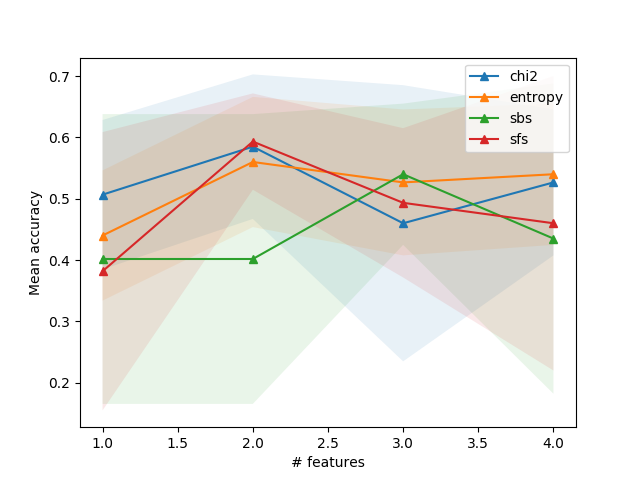
\includegraphics[width=\textwidth]{../plots_with_std_fill/ANNd1.png}
      \caption[]%
      {{\small}}
      \label{fig:ANN_MIAS}
  \end{subfigure}
  \hfill
  \begin{subfigure}[b]{0.475\textwidth}
      \centering
      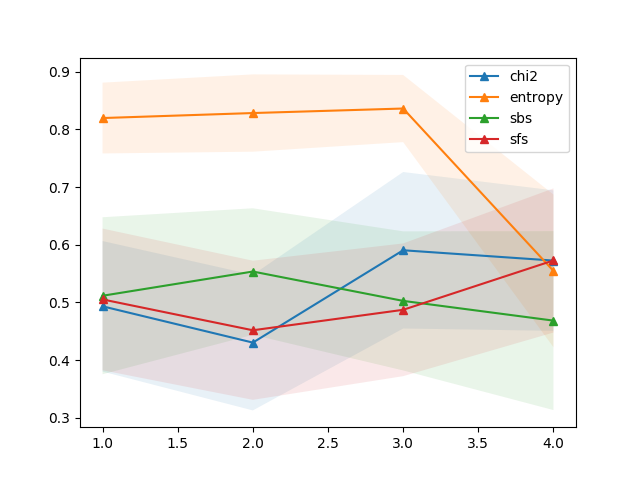
\includegraphics[width=\textwidth]{../plots_with_std_fill/ANNd2.png}
      \caption[]%
      {{\small}}
      \label{fig:ANN_EN}
  \end{subfigure}

  \begin{subfigure}[b]{0.475\textwidth}
      \centering
      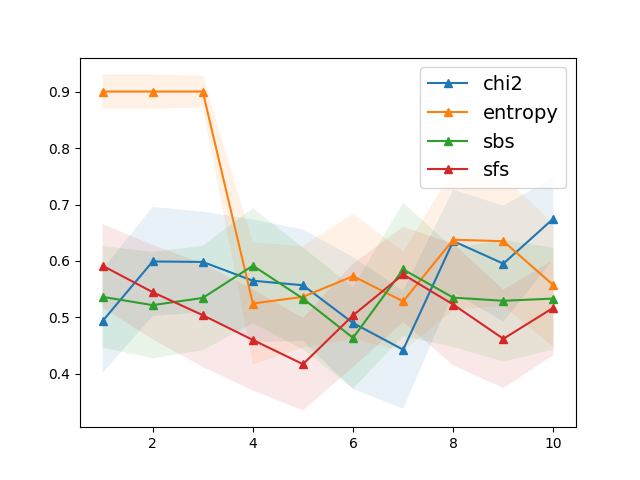
\includegraphics[width=\textwidth]{../plots_with_std_fill/ANNd3.png}
      \caption[]%
      {{\small}}
      \label{fig:ANN_RHH}
  \end{subfigure}
  \quad
  \begin{subfigure}[b]{0.475\textwidth}
      \centering
      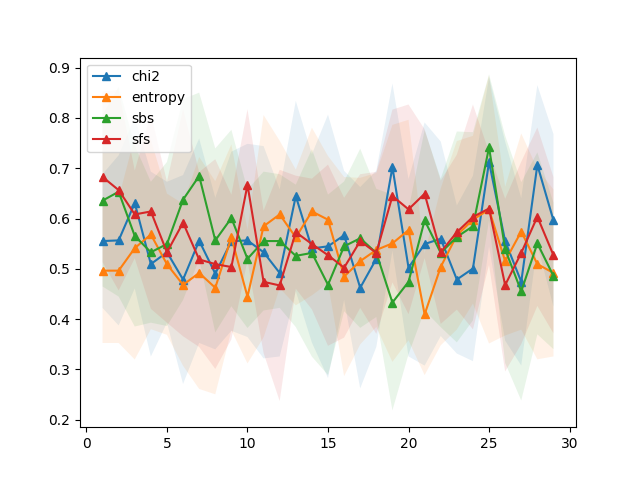
\includegraphics[width=\textwidth]{../plots_with_std_fill/ANNd4.png}
      \caption[]%
      {{\small}}
      \label{fig:ANN_WBCD}
  \end{subfigure}
  \caption[]
  {\small
    Classifier ANN. Each plot corresponds to datasets (a) MIAS, (b) EN, (c) RHH and (d) WBCD. x-axis is number of features, y-axis is mean accuracy achieved by corresponding feature selection method.
  }
  \label{fig:plots_ANN}
\end{figure*}
